% 原印刷104--109页／PDF物理130--135，止于§3.3标题之前.
\subsection[上确界情形]{上确界情形：$L^\infty$}\label{sec:3.2}\index{0003@$L^\infty$传输成本（$L^\infty$ transport cost）|hyperpage}
现在考虑另一个问题：我们不再极小化
\[
K_p(\gamma)=\int|x-y|^p\,d\gamma,
\]
而是希望极小化最大位移，即其$L^\infty$范数. 这一问题最早在\cite{b122}中研究，但这里给出的证明主要取自\cite{b197}.

定义
\begin{equation*}
\begin{aligned}
K_\infty(\gamma)&:=\|x-y\|_{L^\infty(\gamma)}
=\inf\{m\in\mathbb R:|x-y|\le m\text{ 对 }\gamma\text{-几乎处处的 }(x,y)\}\\
&=\max\{|x-y|:(x,y)\in\operatorname{spt}(\gamma)\}
\end{aligned}
\end{equation*}
（最后一个等式把$L^\infty$范数等同于支集上的最大值，由函数$|x-y|$的连续性得到）.

\begin{lemma}\label{obj:3.21}\index{L094@下半连续性（lower semi-continuity）|hyperpage}
对每个$\gamma\in\mathscr P(\Omega\times\Omega)$，当$p\to+\infty$时，量$K_p(\gamma)^{1/p}$单调递增地收敛于$K_\infty(\gamma)$. 特别地，$K_\infty(\gamma)=\sup_{p\ge1}K_p(\gamma)^{1/p}$，且$K_\infty$关于$\mathscr P(\Omega\times\Omega)$中的弱收敛下半连续. 因而，它在紧集$\Pi(\mu,\nu)$上取得极小元.
\end{lemma}
\begin{proof}
众所周知，在任意有限测度空间上，$L^p$范数在$p\to\infty$时收敛于$L^\infty$范数，这里不再证明. 将其用于赋予测度$\gamma$的$\Omega\times\Omega$上的函数$(x,y)\mapsto|x-y|$，便得$K_p(\gamma)^{1/p}\to K_\infty(\gamma)$. 重要的是，这里的收敛为单调收敛；当测度的总质量为一时，确实如此. 在这种情形，对$p<q$，使用Hölder（或Jensen）不等式，得到对每个$f\in L^q(\gamma)$都有
\[
\int|f|^p\,d\gamma\le
\left(\int|f|^q\,d\gamma\right)^{p/q}
\left(\int1\,d\gamma\right)^{1-p/q}
=\left(\int|f|^q\,d\gamma\right)^{p/q}.
\]
取$p$次方根即得$\|f\|_{L^p}\le\|f\|_{L^q}$. 应用于$f(x,y)=|x-y|$，便给出所需的单调性.

由此推出，$K_\infty$是一族关于弱收敛连续的泛函的上确界（由于$\Omega$紧，$K_p$是有界连续函数的积分，而取$p$次方根不破坏连续性）. 作为连续泛函的上确界，它下半连续，结论随之成立.
\end{proof}

现在的目标是分析
\[
\min\{K_\infty(\gamma):\gamma\in\Pi(\mu,\nu)\}
\]
的解，并证明至少有一个极小元$\bar\gamma$由传输映射诱导. 这一映射将解出
\[
\min\{\|\mathrm T-\mathrm{id}\|_{L^\infty(\mu)}:\mathrm T_\#\mu=\nu\}.
\]
这里同样没有唯一性（极小化$L^\infty$准则时，几乎总是如此）；因此定义$O_\infty(\mu,\nu)=\operatorname*{argmin}_{\gamma\in\Pi(\mu,\nu)}K_\infty(\gamma)$，即这一$L^\infty$成本的最优传输方案集合. 注意，由$K_\infty$下半连续，$O_\infty(\mu,\nu)$紧（与$O(\mu,\nu)$类似）. 令$L:=\min\{K_\infty(\gamma):\gamma\in\Pi(\mu,\nu)\}$，可写成
\[
\gamma\in O_\infty(\mu,\nu)\iff\operatorname{spt}(\gamma)\subset\{(x,y):|x-y|\le L\}
\]
（因为任意集中于$|x-y|\le L$的点对上的传输方案$\gamma$，都满足$K_\infty(\gamma)\le L$，从而最优）. 假设$L>0$；否则意味着可以完全不移动便由$\mu$得到$\nu$，即$\mu=\nu$，最优位移为恒等映射.

于是，完全类似于$L^1$情形，可以定义次级变分问题：
\[
\min\{K_2(\gamma):\gamma\in O_\infty(\mu,\nu)\}.
\]
这一问题有解$\bar\gamma$，因为$K_2$关于弱收敛连续，且$O_\infty(\mu,\nu)$紧. 目前不知道这一极小元是否唯一. 同样可以说，$\bar\gamma$还解出
\begin{equation*}
\min\left\{\int_{\Omega\times\Omega}c\,d\gamma:\gamma\in\Pi(\mu,\nu)\right\},\quad
c(x,y)=\begin{cases}|x-y|^2,&|x-y|\le L,\\+\infty,&\text{否则}.\end{cases}
\end{equation*}
论证与$L^1$情形相同. 此外，成本$c$的形式也类似，并且同样下半连续. 因而$\bar\gamma$集中于某个$c$-CM集合$\Gamma\subset\Omega\times\Omega$. 这意味着
\begin{equation}\label{eq:3.5}
\begin{aligned}
&(x_1,y_1),(x_2,y_2)\in\Gamma,\quad |x_1-y_2|,|x_2-y_1|\le L\\
&\hspace{5em}\implies(x_1-x_2)\cdot(y_1-y_2)\ge0.
\end{aligned}
\end{equation}
也可假设$\Gamma\subset\{(x,y):|x-y|\le L\}$. 我们将去掉零测集、获得更好的性质，从而“改进”集合$\Gamma$；随后证明剩下的集合$\widetilde\Gamma$包含在某个映射$\mathrm T$的图中，由此得到结论.

照例假设$\mu\ll\mathscr L^d$. 下面需要回顾Lebesgue点的概念，它是Lebesgue测度所特有的概念.
\Needspace{8\baselineskip}
\begin{sourcebox}{知识回顾：密度点}\label{box:3.2}\index{L089@Lebesgue点（Lebesgue points）|hyperpage}
\begin{definition*}
对于可测集$E\subset\mathbb R^d$，若$x\in\mathbb R^d$满足
\[
\lim_{r\to0}\frac{|E\cap B(x,r)|}{|B(x,r)|}=1,
\]
则称$x$为$E$的Lebesgue点.
\end{definition*}
$E$的Lebesgue点集合记为$\operatorname{Leb}(E)$；众所周知，$|E\setminus\operatorname{Leb}(E)|+|\operatorname{Leb}(E)\setminus E|=0$. 这实际上是一个更一般事实的推论：给定函数$f\in L^1_{\mathrm{loc}}(\mathbb R^d)$，几乎每点$x$都是$f$的Lebesgue点，即$\lim_{r\to0}\fint_{B(x,r)}|f(y)-f(x)|\,dy=0$；这也蕴含$f(x)=\lim_{r\to0}\fint_{B(x,r)}f(y)\,dy$. 将其应用于$f=\mathbbm1_E$，便得到集合的Lebesgue点概念（也称为密度点）.
\end{sourcebox}

\begin{lemma}\label{obj:3.22}\index{0007@$c$-循环单调性（$c$-cyclical monotonicity）|hyperpage}
方案$\bar\gamma$集中于一个$c$-CM集合$\widetilde\Gamma$，使得对每个$(x_0,y_0)\in\widetilde\Gamma$、任意$\varepsilon,\delta>0$、任意单位向量$\xi$以及任意充分小的$r>0$，都存在点$x\in(B(x_0,r)\setminus B(x_0,r/2))\cap C(x_0,\xi,\delta)$和点$y\in B(y_0,\varepsilon)$，使$(x,y)\in\widetilde\Gamma$；其中$C(x_0,\xi,\delta)$为下列凸锥：
\[
C(x_0,\xi,\delta):=\{x:(x-x_0)\cdot\xi>(1-\delta)|x-x_0|\}.
\]
\end{lemma}
\begin{proof}
首先取$c$-CM集合$\Gamma$满足$\bar\gamma(\Gamma)=1$. 令$B_i$为生成$\mathbb R^d$拓扑的一个可数球族（例如，所有球心坐标和半径均为有理数的球）. 考虑
\[
A_i:=(\pi_x)(\Gamma\cap(\Omega\times B_i)),
\]
即所有满足“至少存在一个$y\in B_i$使$(x,y)\in\Gamma$”的点$x$的集合（若将$\bar\gamma$想象为多值映射，就是在$B_i$中至少有一个“像”的点）. 令$N_i:=A_i\setminus\operatorname{Leb}(A_i)$. 此集合为Lebesgue零测集，因而也是$\mu$-零测集. 还有$\mu(\bigcup_iN_i)=0$. 因而可以定义$\widetilde\Gamma:=\Gamma\setminus((\bigcup_iN_i)\times\Omega)$. 由于只去除了$\mu$-零测的点，方案$\bar\gamma$仍集中于$\widetilde\Gamma$. 显然，作为$\Gamma$的子集，$\widetilde\Gamma$仍为$c$-CM，并保持性质\eqref{eq:3.5}.

此外，$\widetilde\Gamma$具有陈述中的性质. 这是因为，至少存在一个球$B_i$包含$y_0$且包含于$B(y_0,\varepsilon)$. 由于$x_0\in A_i$且已经去掉$N_i$，$x_0$就是$A_i$的Lebesgue点. 区域$(B(x_0,r)\setminus B(x_0,r/2))\cap C(x_0,\xi,\delta)$占球$B(x_0,r)$总体积的固定比例（依赖$\delta$），所以当$r\to0$时，$A_i$（以及$\operatorname{Leb}(A_i)$）显然必须与其相交（否则$x_0$就不是Lebesgue点）. 于是只需在$\operatorname{Leb}(A_i)\cap(B(x_0,r)\setminus B(x_0,r/2))\cap C(x_0,\xi,\delta)$中选取一点，就完成了证明.
\end{proof}

\begin{lemma}\label{obj:3.23}
若$(x_0,y_0)$与$(x_0,z_0)$均属于$\widetilde\Gamma$，则$y_0=z_0$（\autoref{fig:3.4}）.
\end{lemma}
\begin{proof}
反设$y_0\ne z_0$. 为固定思路，假设$|x_0-z_0|\le|x_0-y_0|$（特别地，$y_0\ne x_0$，否则$|x_0-z_0|=|x_0-y_0|=0$，从而$z_0=y_0$）.

现在利用$\widetilde\Gamma$的性质，找出$(x,y)\in\widetilde\Gamma$，使$y\in B(y_0,\varepsilon)$且$x\in(B(x_0,r)\setminus B(x_0,r/2))\cap C(x_0,\xi,\delta)$，其中向量$\xi$稍后选定. 将$\widetilde\Gamma$的$c$-CM性质应用于$(x_0,z_0)$与$(x,y)$.

如果能证明$|x-z_0|,|x_0-y|\le L$，就应有
\[
(x-x_0)\cdot(y-z_0)\ge0,
\]
随后可以适当选取$\xi$来得到矛盾. 事实上，$x-x_0$的方向几乎为$\xi$（误差不超过$\delta$），而$y-z_0$的方向几乎为$y_0-z_0$（误差的阶为$\varepsilon/|z_0-y_0|$）. 若选取$\xi$使$\xi\cdot(y_0-z_0)<0$，则对于小的$\delta,\varepsilon$会得到矛盾.

为证明结论，需要保证$|x-z_0|,|x_0-y|\le L$. 计算$|x-z_0|^2$，有
\[
|x-z_0|^2=|x_0-z_0|^2+|x-x_0|^2+2(x-x_0)\cdot(x_0-z_0).
\]
在此和式中，
\begin{equation*}
\begin{aligned}
|x_0-z_0|^2&\le L^2,\qquad |x-x_0|^2\le r^2,\\
2(x-x_0)\cdot(x_0-z_0)&=|x-x_0|(\xi\cdot(x_0-z_0)+O(\delta)).
\end{aligned}
\end{equation*}
现在假设以下情况之一成立：或者选取$\xi$使$\xi\cdot(x_0-z_0)<0$，或者$|x_0-z_0|^2<L^2$. 两种情形中，只要$r,\delta$充分小，都能得到$|x-z_0|\le L$. 第一种情形下，因为$|x-x_0|\ge r/2$，有一个$r$阶负项和一个$r^2$阶正项；第二种情形下，在$|x_0-z_0|^2<L^2$上加上若干$r$或$r^2$阶的项.

类似地，对于$|x_0-y|$，有
\[
|x_0-y|^2=|x_0-x|^2+|x-y|^2+2(x_0-x)\cdot(x-y).
\]
这三项满足
\begin{equation*}
\begin{aligned}
|x_0-x|^2&\le r^2,\qquad |x-y|^2\le L^2,\\
2(x_0-x)\cdot(x-y)&=|x-x_0|(-\xi\cdot(x_0-y_0)+O(\delta+\varepsilon+r)).
\end{aligned}
\end{equation*}
这时，或者有$|x_0-y_0|<L$（从而当$\varepsilon,\delta$充分小时保证$|x_0-y|<L$），或者需要施加$\xi\cdot(y_0-x_0)<0$.

注意，施加$\xi\cdot(y_0-x_0)<0$和$\xi\cdot(x_0-z_0)<0$，便自动得到$\xi\cdot(y_0-z_0)<0$，即得出矛盾所需的条件. 令$\mathbf v=y_0-x_0$、$\mathbf w=x_0-z_0$. 如果能够找出$\xi$使$\xi\cdot \mathbf v<0$且$\xi\cdot \mathbf w<0$，证明就完成了. 两个向量$\mathbf v,\mathbf w$何时不存在与二者标量积都为负的向量$\xi$？唯一的情形是它们方向相反. 但这意味着$x_0,y_0,z_0$共线，且$z_0$位于$x_0$与$y_0$之间（因为假设$|x_0-z_0|\le|x_0-y_0|$）. 若$z_0$与$y_0$不同，就应有$|x_0-z_0|<L$. 因而此时不必检验$\xi\cdot(x_0-z_0)<0$. 只需一个向量$\xi$满足$\xi\cdot(y_0-x_0)<0$且$\xi\cdot(y_0-z_0)<0$，但$y_0-x_0$与$y_0-z_0$方向相同，故只需与一个方向的标量积为负，许多$\xi$都能保证这一点. 例如取$\xi=-(y_0-x_0)/|y_0-x_0|$.
\end{proof}

\begin{figure}[htbp]\centering
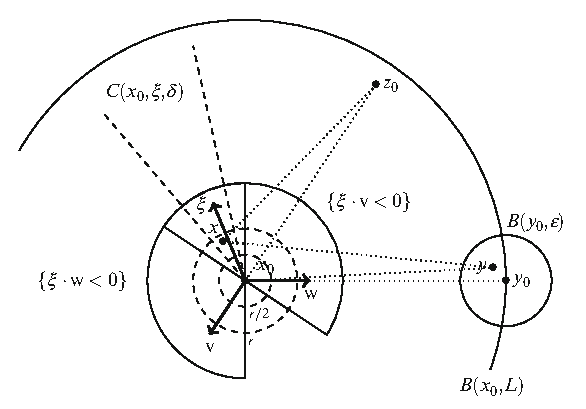
\includegraphics[width=.82\textwidth]{assets/ch03-fig-3-4.pdf}
\caption{\autoref{obj:3.23}证明中的点.}\label{fig:3.4}
\end{figure}

\begin{theorem}\label{obj:3.24}\index{E058@最优映射的存在性（existence of an optimal map）|hyperpage}
次级变分问题
\[
\min\{K_2(\gamma):\gamma\in O_\infty(\mu,\nu)\}
\]
有唯一解$\bar\gamma$，它由传输映射$\mathrm T$诱导，而且该映射是问题
\[
\min\{\|\mathrm T-\mathrm{id}\|_{L^\infty(\mu)};\ \mathrm T_\#\mu=\nu\}
\]
的最优传输.
\end{theorem}
\begin{proof}
已知$\bar\gamma$集中于一个具有若干有用性质的集合$\widetilde\Gamma$. \autoref{obj:3.23}说明$\widetilde\Gamma$包含在一个图中，因为对任意$x_0$，满足$(x_0,y_0)\in\widetilde\Gamma$的点$y_0$至多一个. 将这一点$y_0$视为$x_0$的像，记为$\mathrm T(x_0)$，则$\bar\gamma=\gamma_{\mathrm T}$. 将这一$L^\infty$问题的“Monge”形式与其在方案$\gamma$上的Kantorovich形式作通常的比较，即得$\mathrm T$的最优性. 唯一性由标准论证得到（极小元的凸组合仍应为极小元，因此可以使用\autoref{obj:1.19}中的证明）.
\end{proof}
